\documentclass[12pt, oneside]{amsart}   	% use "amsart" instead of "article" for AMSLaTeX format
\usepackage[margin=1in]{geometry}                		% See geometry.pdf to learn the layout options. There are lots.
\geometry{letterpaper}                   		% ... or a4paper or a5paper or ... 
%\geometry{landscape}                		% Activate for for rotated page geometry
\usepackage[parfill]{parskip}    		% Activate to begin paragraphs with an empty line rather than an indent
\usepackage{graphicx}				% Use pdf, png, jpg, or eps§ with pdflatex; use eps in DVI mode
								% TeX will automatically convert eps --> pdf in pdflatex		
\usepackage{amssymb,hyperref}
\usepackage{listings}

\title{Week 3: Source Files and Packages}
\author{Thomas Elliott}
\date{\today}							% Activate to display a given date or no date

\begin{document}
\maketitle
\lstset{language=R}

\section{Source Files}

Source files function exactly like Stata Do files. They are plain text files containing lists of commands to execute. Source files typically end with the file extension \texttt{.R}. To run a source file within R, you use the \texttt{source()} command. For example, say we had the following commands in a source file we've saved as ``my-source-file.R'':

\begin{lstlisting}
x<-c(1,2,3,4,5)
y<-c(6,7,8,9,10)

z<-x*y

print(z)
\end{lstlisting}

We can run all the commands in the source file with the following command:

\begin{lstlisting}
> source("my-source-file.R")
[1]  6 14 24 36 50
\end{lstlisting}

By default, sourcing a source file will not output the commands it is running. It will, however, output any messages, warnings, errors, and print statements. So in the source file above, the only thing that gets output to the console is the contents of z from the \texttt{print(z)} command. If you want to see the commands it is running, you can supply the \texttt{echo=TRUE} argument to the source command:

\begin{lstlisting}
> source('my-source-file.R', echo=TRUE)

> x<-c(1,2,3,4,5)

> y<-c(6,7,8,9,10)

> z<-x*y

> print(z)
[1]  6 14 24 36 50
\end{lstlisting}

This is another area where RStudio is particularly helpful. As you've noticed by now, RStudio has four panes to show various information, outputs, etc. One of these panes is for working on source files (see Figure \ref{fig:source}. This pane will do syntax highlighting, which means it can tell the difference between different parts of the code and display the text in different colors to help with reading your code. RStudio's source editor is also smart enough to figure out how things should be indented, and so will automatically indent lines of code the appropriate amount to facilitate reading your code. The source pane can have multiple source files open at once, and will display tabs to change between them. While you are working in the source pane, there are keyboard shortcuts to run the line your cursor is on in the console, making checking that your code works really easy. 

\begin{figure}[t]
\caption{The Source Pane}
\centering
\label{fig:source}
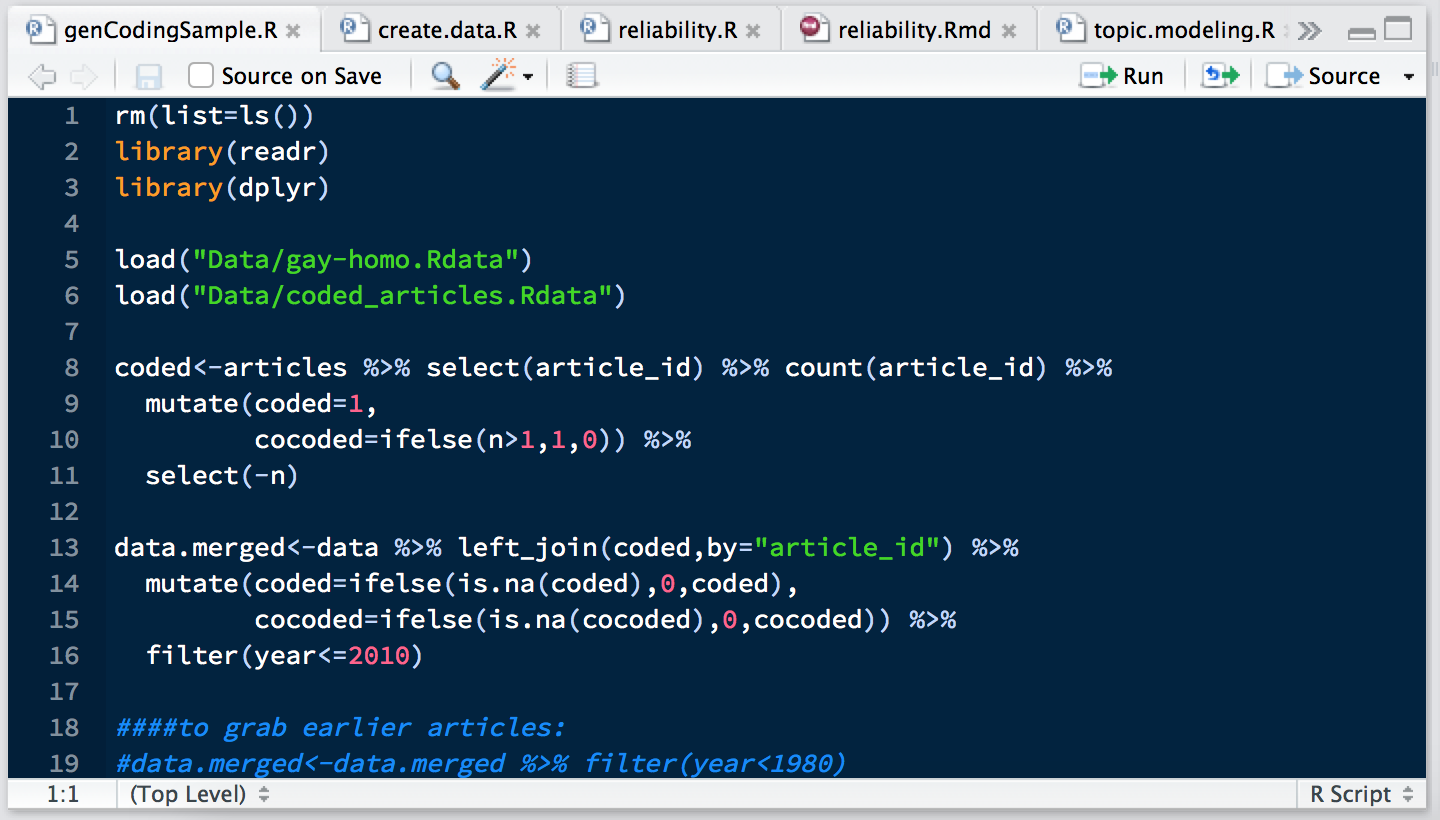
\includegraphics[width=0.75\textwidth]{source_pane}
\end{figure}

\subsection{Logging Output}

One unfortunate aspect of R is that it's logging capabilities are not as intuitive as Stata's. You can redirect console output to a text file using the \texttt{sink()} command, but it is easy mess things up with sink --- again, R requires more user vigilance than Stata does. Sink works by creating a new output stream - think of what gets printed to the console as originating from a lake or dam. The console is one stream from the lake, but you can, on the fly, create new ones to redirect the output. To use \texttt{sink()} you insert the command where you want to start redirecting the output, supplying a filename as an argument for the text file where the output will be saved. By default, redirecting output means the output will NOT show up on the console, only the text file. If you want the output to show up in both, you can supply the \texttt{split=TRUE} argument. To stop redirecting the output, you can type \texttt{sink()} with no arguments, or \texttt{sink(NULL)}, which is equivalent. This closes the current redirection of the output. As an example, if we wanted to source our source file, echoing the commands, and outputting the results to both the console and a text file, we would type:

\begin{verbatim}
> sink("test.txt",split=TRUE)
> source('my-source-file.R', echo=TRUE)

> x<-c(1,2,3,4,5)

> y<-c(6,7,8,9,10)

> z<-x*y

> print(z)
[1]  6 14 24 36 50
> sink()
\end{verbatim}

Now, the tricky thing with sink is that you can create new redirections while you are already redirecting output. For example, say you sink to a text file called ``cleaning-log.txt" for a source file that cleans your data. You could, while that sink is still active, create a new sink that redirects output to ``cleaning-errors.txt" where you output any errors the cleaning program found. At this point, typing \texttt{sink(NULL)} closes the redirection to ``cleaning-errors.txt'' and returns to the redirection to ``cleaning-log.txt''. As a result, you should pay careful attention to what redirections of output you already have in place as you write code in R. You can query the number of diversions of output with the command \texttt{sink.number()}, which returns the number of diversions that are currently active. 

\section{Packages}

In Stata you can install third-party functions, often stored in ado files, to extend the capabilities of Stata. You can do the same thing with R using packages. In fact, what makes R so powerful is the richness of its packages archive. When you installed R, it came with some packages that were also installed and these are automatically loaded whenever you start R. Examples of these packages include the \texttt{stats} package, which contains the bulk of the basic statistical analysis functions, including \texttt{lm()}; and the \texttt{utils} package, which contains a bunch of functions for working in R, including the \texttt{help()} functions discussed last week. However, there are some packages you may want to use that are not automatically installed and loaded when you start R. Two such packages I strongly recommend installing and using are the \texttt{dplyr} and \texttt{tidyr} packages, which makes data wrangling much easier than base R. Once you know the name of the package you want to install, you can install it using the \texttt{install.packages()} command in R:

\begin{verbatim}
install.packages(c("dplyr","tidyr"))
\end{verbatim}

If you are only installing one package, you can just enter the name of the package with quotes as an argument to \texttt{install.packages()}. However, if you want to install more than one package at once, you'll need to supply a character vector. You do this with the \texttt{c()} function, which combines values into a vector. 

If this is the first time you are installing packages and you are not using RStudio, you will be asked which CRAN mirror to use. CRAN is the archive which stores the official versions of R packages, and it is from this archive that packages are downloaded and updated. You will want to choose a mirror that is close to you - you are more likely to get a faster connection to servers that are geographically closer to you than farther away. RStudio hosts its own CRAN mirror and so will automatically use this when installing packages, which is fine. 

If you do not have administer privileges on the user you are currently logged into, you will likely get a message saying R cannot write to a folder where it defaults to installing packages. It should ask if you would like R to, instead, install to a folder in your user folder - this is fine to do, but means that the installed packages will not be accessible to other users on your computer. They will have to install the packages themselves, which is fine. 

You only need to install a package once, but in order to use the functions in the package during a R session, you need to tell R to load the package into the workspace. You do this with the \texttt{library()} function. Once you've installed \texttt{dplyr} and \texttt{tidyr}, you can load them into your session with:

\begin{verbatim}
library(tidyr)
library(dplyr)
Attaching package: `dplyr'

The following objects are masked from `package:stats':

    filter, lag

The following objects are masked from `package:base':

    intersect, setdiff, setequal, union
\end{verbatim}  

Notice that some packages will output messages when they are loaded. In the above example, dplyr contains functions that are named the same as functions in other packages that are already loaded. Loaded packages stack, so that the most recently loaded package takes precedence over older loaded packages. When you use a function and R goes to find where that function is located, it traverses down this stack and will return the first function definition it finds. Thus, using the \texttt{filter()} function after loading \texttt{dplyr} will always return \texttt{dplyr}'s version of \texttt{filter()}, not \texttt{stats}'. This is \textit{usually} not a problem, as package developers are usually good about not using the same names for functions as other common functions, but it is still something to pay attention to - the load order is important for packages. It is possible to use functions that have been masked by another package, by telling R which package it should be looking for the function in. For example, to use \texttt{stats}' filter function, you would type \texttt{stats::filter()} --- the \texttt{stats::} is telling R to look in the stats package for the filter function. 

\subsection{Updating Packages}

You can check for updates to installed packages with the \texttt{update.packages()} function. This will check the version number of your installed packages with the version number of the package on your CRAN mirror and will offer to download any newer packages it finds. 

\subsection{Creating Your Own Packages}

Creating your own packages is a fairly easy process, made even easier by RStudio. I won't go into details about how to create packages here, but I highly recommend Hadley Wickham's book on creating R packages with RStudio, which you can read for free online here: \url{http://r-pkgs.had.co.nz}

\end{document}  